\documentclass[11pt]{article}

% ── Packages ────────────────────────────────────────────────────────────────
\usepackage[utf8]{inputenc}
\usepackage[T1]{fontenc}
\usepackage[margin=1in]{geometry}
\usepackage{amsmath,amssymb}
\usepackage{cancel}
\usepackage{graphicx}
\graphicspath{{figures/}}
\usepackage{subcaption}
\usepackage{float}
\usepackage{placeins}
\usepackage{booktabs}
\usepackage{tabularx}
\usepackage{siunitx}
\usepackage{xcolor}
\usepackage{tikz}
\usetikzlibrary{arrows.meta,bending,calc}
\usepackage{listings}
\usepackage{microtype}
\usepackage{needspace}
\let\oldsection\section
\renewcommand{\section}{\Needspace{12\baselineskip}\oldsection}   % keep problem headings off page bottoms
\usepackage{hyperref}
\hypersetup{
    colorlinks = true,
    linkcolor  = blue!50!black,
    citecolor  = black,
    urlcolor   = blue!50!black,
}
\usepackage{cleveref}

% ── Code listing style ─────────────────────────────────────────────────────
\definecolor{codebg}{RGB}{247,247,250}
\definecolor{codekeyword}{RGB}{0,33,165}
\definecolor{codecomment}{RGB}{110,110,110}
\definecolor{codestring}{RGB}{160,30,30}

\lstdefinestyle{pythonstyle}{
    language=Python,
    backgroundcolor=\color{codebg},
    basicstyle=\ttfamily\scriptsize,
    keywordstyle=\color{codekeyword}\bfseries,
    commentstyle=\color{codecomment}\itshape,
    stringstyle=\color{codestring},
    numbers=left,
    numberstyle=\tiny\color{gray},
    numbersep=8pt,
    frame=single,
    rulecolor=\color{black!20},
    breaklines=true,
    breakatwhitespace=false,
    showstringspaces=false,
    tabsize=4,
    captionpos=b,
    columns=fullflexible,
    keepspaces=true,
    extendedchars=true,
    literate=
        {—}{{---}}1
}
\lstset{style=pythonstyle}

% ── Program output style ───────────────────────────────────────────────────
\lstdefinestyle{outputstyle}{
    language={},
    backgroundcolor=\color{codebg},
    basicstyle=\ttfamily\small,
    frame=single,
    rulecolor=\color{black!20},
    breaklines=true,
    columns=fullflexible,
    keepspaces=true,
    numbers=none,
}
\newcommand{\programoutput}[2][]{\lstinputlisting[style=outputstyle,#1]{#2}}

% ── Colors used in the figures (match the handwritten diagrams) ────────────
\definecolor{hwpurple}{RGB}{90,45,145}
\definecolor{hwmagenta}{RGB}{230,0,200}
\definecolor{hwblue}{RGB}{20,70,190}
\definecolor{hwred}{RGB}{225,30,30}
\definecolor{hwgreen}{RGB}{0,130,70}

% ── Vector notation (underbar, matching handwritten convention) ────────────
\newcommand{\vect}[1]{\underline{#1}}
\newcommand{\ivect}[1]{{}^{I}\underline{#1}}   % inertial-frame vector, e.g. {}^I v
\newcommand{\Iddt}{{}^{I}\!\frac{d}{dt}}         % inertial time derivative
\newcommand{\En}{\mathcal{E}}                   % specific mechanical energy

% ── Divider page (used for the appendix section-break) ─────────────────────
\newcommand{\dividerpage}[3]{%
    \clearpage
    \thispagestyle{empty}
    \begin{center}
        \vspace*{\fill}
        {\Huge\bfseries #1\par}
        \vspace{1cm}
        {\Large #2\par}
        \vspace{1.5cm}
        {\normalsize #3\par}
        \vspace*{\fill}
    \end{center}
    \clearpage
}

% ── Source code link ────────────────────────────────────────────────────────
\newcommand{\repolink}{\url{https://github.com/PabloCoralDev/Astrodynamics-HW3}}

\title{EAS4510: Homework Assignment \#3}
\author{Pablo Coral}
\date{\today}

\begin{document}

% ── Cover page ───────────────────────────────────────────────────────────
\pagenumbering{roman}
\begin{titlepage}
    \centering
    \vspace*{4cm}
    {\LARGE\bfseries EAS4510: Homework Assignment \#3\par}
    \vspace{0.8cm}
    {\Large Chapter 2: The Orbit in Space\par}
    \vspace{1.5cm}
    {\Large Pablo Coral\par}
    \vspace{0.5cm}
    {\large \today\par}
    \vspace{1cm}
    {\normalsize All code and sources can be found in: \repolink\par}
    \vfill
\end{titlepage}
\clearpage
\pagenumbering{arabic}
\setcounter{page}{1}

\section{Problem 1}
\label{sec:problem1}

The function \texttt{get\_orbital\_params} (\cref{app:p1-code}) computes the six orbital elements from the position $[\vect{r}]_I$ and inertial velocity $[\ivect{V}]_I$ in PCI coordinates and the gravitational parameter $\mu$. The output is $\Theta = [a,\ e,\ \Omega,\ i,\ \omega,\ \nu]^T$, with angles in degrees. The specific angular momentum, eccentricity vector, and line of nodes are computed first:
\begin{equation}
\ivect{h} = \vect{r}\times\ivect{V}, \qquad
p = \frac{h^2}{\mu}, \qquad
\vect{e} = \frac{\ivect{V}\times\ivect{h}}{\mu} - \frac{\vect{r}}{r}, \qquad
a = \frac{p}{1-e^2}, \qquad
\vect{n} = \vect{I}_z\times\ivect{h}.
\label{eq:p1-vectors}
\end{equation}
Each angle is a four-quadrant inverse tangent, $\tan^{-1}(A, B)$. The arguments $A$ and $B$ are stored in a dictionary together with a flag that indicates whether the angle needs a correction (\cref{tab:p1-angles}):
\begin{equation}
\theta = \tan^{-1}(A, B), \qquad
\text{if correction and } \theta<0:\ \theta = \theta + 2\pi.
\end{equation}

\begin{table}[H]
\centering
\renewcommand{\arraystretch}{1.3}
\begin{tabular}{@{}cccc@{}}
\toprule
Angle & $A$ & $B$ & Correction \\
\midrule
$\Omega$ & $\vect{n}\cdot\vect{I}_y$ & $\vect{n}\cdot\vect{I}_x$ & True \\
$i$ & $\ivect{h}\cdot\left[\vect{n}\times\vect{I}_z\right]$ & $\|\vect{n}\|\left[\ivect{h}\cdot\vect{I}_z\right]$ & False \\
$\omega$ & $\vect{e}\cdot\left[\ivect{h}\times\vect{n}\right]$ & $\|\ivect{h}\|\left[\vect{e}\cdot\vect{n}\right]$ & True \\
$\nu$ & $\vect{r}\cdot\left[\ivect{h}\times\vect{e}\right]$ & $\|\ivect{h}\|\left[\vect{r}\cdot\vect{e}\right]$ & True \\
\bottomrule
\end{tabular}
\caption{Inverse tangent arguments and correction flag for each angle, as stored in the code.}
\label{tab:p1-angles}
\end{table}

\FloatBarrier

\section{Problem 2}
\label{sec:problem2}

The function \texttt{get\_velocity\_position\_vector} (\cref{app:p2-code}) performs the inverse operation. It takes $\Theta$ and $\mu$ and returns $[\vect{r}]_I$ and $[\ivect{V}]_I$ in PCI coordinates. The perifocal basis is reached from the inertial basis by three rotations in a 3--1--3 sequence (\cref{fig:p2}):
\begin{enumerate}
    \item A 3-rotation by $\Omega$ about $\vect{I}_z$ aligns $\vect{I}_x$ with the line of nodes $\vect{n}$.
    \item A 1-rotation by $i$ about $\vect{n}$ aligns $\vect{I}_z$ with $\ivect{h}$.
    \item A 3-rotation by $\omega$ about $\ivect{h}$ aligns $\vect{I}_x$ with $\vect{e}$, which points to periapsis.
\end{enumerate}

\begin{figure}[H]
\centering
% Problem 2: 3-1-3 rotation, inertial -> perifocal (drawn with Omega = 60, i = 35, omega = 50 deg)
% oblique projection: x -> (-0.9,-0.7), y -> (1.4,0), z -> (0,1.4)
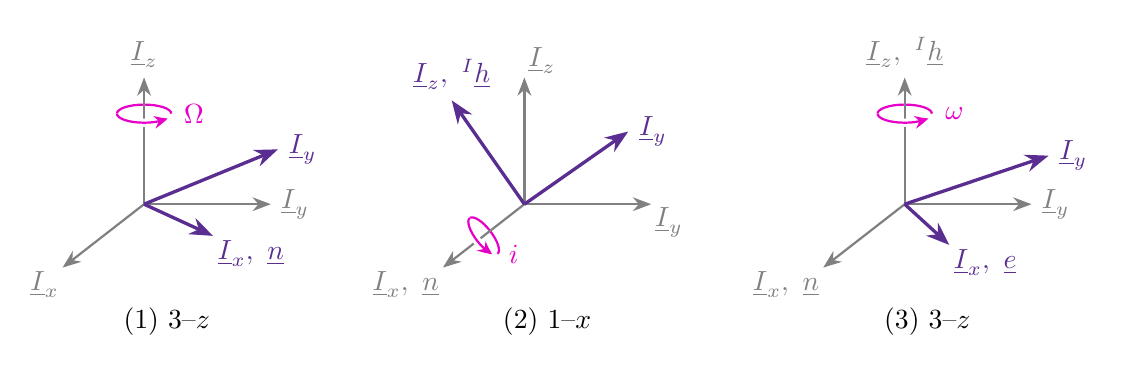
\begin{tikzpicture}[>=Stealth, scale=1.15]
    \tikzset{old/.style={->,gray,thick}, new/.style={->,hwpurple,very thick},
        rot/.style={hwmagenta,thick},
        rotfront/.style={rot,-{Stealth[length=5pt,width=4.5pt,bend]},preaction={draw,white,line width=3pt,-}}}

    % ---------- (1) 3-rotation by Omega about I_z ----------
    \begin{scope}
        \draw[rot] (0.3,1.0) arc[start angle=0, end angle=180, x radius=0.3, y radius=0.1];
        \draw[old] (0,0) -- (-0.9,-0.7) node[below left,inner sep=1pt] {$\vect{I}_x$};
        \draw[old] (0,0) -- (1.4,0) node[right] {$\vect{I}_y$};
        \draw[old] (0,0) -- (0,1.4) node[above] {$\vect{I}_z$};
        \draw[new] (0,0) -- (0.762,-0.35) node[below right,inner sep=1pt] {$\vect{I}_x,\ \vect{n}$};
        \draw[new] (0,0) -- (1.479,0.606) node[right] {$\vect{I}_y$};
        \draw[rotfront] (-0.3,1.0) arc[start angle=180, end angle=330, x radius=0.3, y radius=0.1];
        \node[hwmagenta] at (0.55,1.0) {$\Omega$};
        \node at (0.25,-1.3) {(1) 3--$z$};
    \end{scope}

    % ---------- (2) 1-rotation by i about n ----------
    \begin{scope}[shift={(4.2,0)}]
        \draw[rot,shift={(-0.45,-0.35)},rotate=127.9] (-0.25,0) arc[start angle=180, end angle=360, x radius=0.25, y radius=0.09];
        \draw[old] (0,0) -- (-0.9,-0.7) node[below left,inner sep=1pt] {$\vect{I}_x,\ \vect{n}$};
        \draw[old] (0,0) -- (1.4,0) node[below right,inner sep=1pt] {$\vect{I}_y$};
        \draw[old] (0,0) -- (0,1.4) node[above right,inner sep=1pt] {$\vect{I}_z$};
        \draw[new] (0,0) -- (-0.803,1.147) node[above] {$\vect{I}_z,\ \ivect{h}$};
        \draw[new] (0,0) -- (1.147,0.803) node[right] {$\vect{I}_y$};
        \draw[rotfront,shift={(-0.45,-0.35)},rotate=127.9] (0.25,0) arc[start angle=0, end angle=150, x radius=0.25, y radius=0.09];
        \node[hwmagenta] at (-0.12,-0.55) {$i$};
        \node at (0.25,-1.3) {(2) 1--$x$};
    \end{scope}

    % ---------- (3) 3-rotation by omega about h ----------
    \begin{scope}[shift={(8.4,0)}]
        \draw[rot] (0.3,1.0) arc[start angle=0, end angle=180, x radius=0.3, y radius=0.1];
        \draw[old] (0,0) -- (-0.9,-0.7) node[below left,inner sep=1pt] {$\vect{I}_x,\ \vect{n}$};
        \draw[old] (0,0) -- (1.4,0) node[right] {$\vect{I}_y$};
        \draw[old] (0,0) -- (0,1.4) node[above] {$\vect{I}_z,\ \ivect{h}$};
        \draw[new] (0,0) -- (0.493,-0.45) node[below right,inner sep=1pt] {$\vect{I}_x,\ \vect{e}$};
        \draw[new] (0,0) -- (1.589,0.536) node[right] {$\vect{I}_y$};
        \draw[rotfront] (-0.3,1.0) arc[start angle=180, end angle=330, x radius=0.3, y radius=0.1];
        \node[hwmagenta] at (0.55,1.0) {$\omega$};
        \node at (0.25,-1.3) {(3) 3--$z$};
    \end{scope}
\end{tikzpicture}

\caption{3--1--3 rotation of the inertial basis $\{\vect{I}_x,\vect{I}_y,\vect{I}_z\}$ into the perifocal basis: rotation by $\Omega$ about $\vect{I}_z$, by $i$ about $\vect{n}$, then by $\omega$ about $\ivect{h}$. In each step the axes are gray before and purple after the rotation. Each axis keeps its name and is labeled with the vector it is aligned with.}
\label{fig:p2}
\end{figure}

The position and inertial velocity are first written in the perifocal basis,
\begin{equation}
r = \frac{a(1-e^2)}{1+e\cos\nu}, \qquad
\left[\vect{r}\right]_{\text{perifocal}} = \begin{bmatrix} r\cos\nu \\ r\sin\nu \\ 0 \end{bmatrix}, \qquad
\left[\ivect{V}\right]_{\text{perifocal}} = \sqrt{\frac{\mu}{p}}\begin{bmatrix} -\sin\nu \\ e+\cos\nu \\ 0 \end{bmatrix},
\end{equation}
and then transformed to PCI coordinates:
\begin{equation}
\setlength{\fboxsep}{8pt}
\boxed{
\begin{gathered}
\left[\vect{r}\right]_{\text{inertial}} = T^{\text{inertial}}_{\text{perifocal}}\left[\vect{r}\right]_{\text{perifocal}}, \qquad
\left[\ivect{V}\right]_{\text{inertial}} = T^{\text{inertial}}_{\text{perifocal}}\left[\ivect{V}\right]_{\text{perifocal}} \\[10pt]
T^{\text{inertial}}_{\text{perifocal}} = R_3(\Omega)\,R_1(i)\,R_3(\omega)
\end{gathered}
}
\end{equation}

\FloatBarrier

\section{Problem 3}
\label{sec:problem3}

The angles $\Omega$, $i$, $\omega$, and $\nu$ are all computed with a four-quadrant inverse tangent (\cref{tab:p1-angles}), which is undefined at $\tan^{-1}(0,0)$. This occurs in the following cases.
\begin{enumerate}
    \item Circular orbit, $e=0$, so $\vect{e}=\vect{0}$. The true anomaly is measured from periapsis, but a circle has no periapsis:
    \begin{equation}
    \nu = \tan^{-1}\!\left(\vect{r}\cdot\left[\ivect{h}\times\vect{e}\right],\ h\left[\vect{r}\cdot\vect{e}\right]\right) = \tan^{-1}(0,0).
    \end{equation}
    \item Equatorial orbit, $i=0$. Since $\ivect{h}\parallel\vect{I}_z$, the line of nodes vanishes, $\vect{n} = \vect{I}_z\times\ivect{h} = \vect{0}$, and
    \begin{equation}
    \Omega = \tan^{-1}\!\left(\vect{n}\cdot\vect{I}_y,\ \vect{n}\cdot\vect{I}_x\right) = \tan^{-1}(0,0).
    \end{equation}
    \item Cases 1 and 2 imply that $\omega$ is undefined if the orbit is equatorial ($\vect{n}=\vect{0}$) or circular ($\vect{e}=\vect{0}$):
    \begin{equation}
    \omega = \tan^{-1}\!\left(\vect{e}\cdot\left[\ivect{h}\times\vect{n}\right],\ h\left[\vect{e}\cdot\vect{n}\right]\right) = \tan^{-1}(0,0).
    \end{equation}
\end{enumerate}
The remaining elements are summarized with these cases in \cref{tab:p3}.

\begin{table}[H]
\centering
\renewcommand{\arraystretch}{1.3}
\begin{tabularx}{\textwidth}{@{}llX@{}}
\toprule
Element & Not defined when & Why \\
\midrule
$a$ & $e=1$ (parabolic) & $a = p/(1-e^2) = p/0 \rightarrow \infty$; not physically meaningful for an open orbit \\
$e$ & always defined & $e\in[0,\infty)$ \\
$i$ & $\ivect{h}=\vect{0}$ & no orbit plane; still defined for $\vect{n}=\vect{0}$ \\
$\Omega$ & $i=0$ (equatorial) & $\vect{n}=\vect{0}$ \\
$\omega$ & $i=0$ or $e=0$ & $\vect{n}=\vect{0}$ or $\vect{e}=\vect{0}$ \\
$\nu$ & $e=0$ (circular) & $\vect{e}=\vect{0}$; no periapsis \\
\bottomrule
\end{tabularx}
\caption{Cases where each orbital element is not well defined.}
\label{tab:p3}
\end{table}

\FloatBarrier

\section{Problem 4}
\label{sec:problem4}

The specific angular momentum $\ivect{h}$, the eccentricity vector $\vect{e}$, and the line of nodes $\vect{n}$ are shown to be constant in the inertial frame. The planet is treated as an inertial reference frame and all distances are measured from its center, so no extra transport theorem terms appear.

\subsection*{(a) Specific angular momentum}

Differentiating $\ivect{h}$ in the inertial frame,
\begin{equation}
\ivect{h} = \vect{r}\times\ivect{V}, \qquad
\Iddt\left(\ivect{h}\right) = \Iddt(\vect{r})\times\ivect{V} + \vect{r}\times\Iddt\left(\ivect{V}\right) = \underbrace{\ivect{V}\times\ivect{V}}_{\vect{0}} + \vect{r}\times\ivect{a},
\end{equation}
where the first term vanishes because the cross product of collinear vectors is zero. From the two-body differential equation,
\begin{equation}
\ivect{a} + \frac{\mu}{r^3}\vect{r} = \vect{0} \;\Rightarrow\; \ivect{a} = -\frac{\mu}{r^3}\vect{r},
\qquad\therefore\quad
\vect{0} + \vect{r}\times\left(-\frac{\mu}{r^3}\vect{r}\right) = -\frac{\mu}{r^3}\left(\vect{r}\times\vect{r}\right) = \vect{0},
\end{equation}
\begin{equation}
\boxed{\Iddt\left(\ivect{h}\right) = \vect{0}}
\end{equation}

\subsection*{(b) Eccentricity vector}

The eccentricity vector is split into two terms,
\begin{equation}
\vect{e} = \underbrace{\frac{\ivect{V}\times\ivect{h}}{\mu}}_{A} - \underbrace{\frac{\vect{r}}{r}}_{B},
\end{equation}
and each is differentiated separately. If $\Iddt(\vect{e}) = \vect{0}$, then $\vect{e}$ is fixed in time.

\paragraph{A:} Using the result of (a),
\begin{equation}
\begin{aligned}
\frac{1}{\mu}\Iddt\left(\ivect{V}\times\ivect{h}\right) &= \frac{1}{\mu}\left[\Iddt\left(\ivect{V}\right)\times\ivect{h} + \ivect{V}\times\underbrace{\Iddt\left(\ivect{h}\right)}_{\vect{0}\text{ from (a)}}\right] \\
&= \frac{1}{\mu}\left(\ivect{a}\times\ivect{h}\right)
= \frac{1}{\mu}\left(-\frac{\mu}{r^3}\vect{r}\times\ivect{h}\right) = -\frac{1}{r^3}\left(\vect{r}\times\ivect{h}\right).
\end{aligned}
\end{equation}
Expanding $\ivect{h}$ and applying the vector triple product, $\vect{a}\times(\vect{b}\times\vect{c}) = (\vect{a}\cdot\vect{c})\vect{b} - (\vect{a}\cdot\vect{b})\vect{c}$ with $\vect{a}=\vect{b}=\vect{r}$ and $\vect{c}=\ivect{V}$,
\begin{equation}
-\frac{1}{r^3}\left(\vect{r}\times\left(\vect{r}\times\ivect{V}\right)\right)
= -\frac{1}{r^3}\left[\left(\vect{r}\cdot\ivect{V}\right)\vect{r} - r^2\,\ivect{V}\right],
\qquad
\therefore\quad \Iddt(A) = \frac{\ivect{V}}{r} - \frac{\left(\vect{r}\cdot\ivect{V}\right)}{r^3}\vect{r}.
\end{equation}

\paragraph{B:} Applying the quotient rule with $u=\vect{r}$, $u'=\ivect{V}$, $w=r$, and $w'=\dot r = \ivect{V}\cdot\dfrac{\vect{r}}{r} = \dfrac{\left(\vect{r}\cdot\ivect{V}\right)}{r}$,
\begin{equation}
\Iddt\left(\frac{\vect{r}}{r}\right) = \frac{\ivect{V}\,r - \dot r\,\vect{r}}{r^2}
= \frac{\ivect{V}}{r} - \frac{\dot r}{r^2}\vect{r}
= \frac{\ivect{V}}{r} - \frac{\left(\vect{r}\cdot\ivect{V}\right)}{r^3}\vect{r}.
\end{equation}
Subtracting the two results,
\begin{equation}
\Iddt(\vect{e}) = \Iddt(A) - \Iddt(B)
= \left[\frac{\ivect{V}}{r} - \frac{\left(\vect{r}\cdot\ivect{V}\right)}{r^3}\vect{r}\right]
- \left[\frac{\ivect{V}}{r} - \frac{\left(\vect{r}\cdot\ivect{V}\right)}{r^3}\vect{r}\right],
\end{equation}
\begin{equation}
\boxed{\Iddt(\vect{e}) = \vect{0}}
\end{equation}
Therefore, $\vect{e}$ is fixed in the inertial frame.

\subsection*{(c) Line of nodes}

Since $\vect{I}_z$ is fixed in the inertial frame and $\Iddt\left(\ivect{h}\right)=\vect{0}$ from (a),
\begin{equation}
\vect{n} = \vect{I}_z\times\ivect{h}, \qquad
\Iddt(\vect{n}) = \underbrace{\Iddt\left(\vect{I}_z\right)}_{\vect{0}}\times\ivect{h} + \vect{I}_z\times\underbrace{\Iddt\left(\ivect{h}\right)}_{\vect{0}},
\qquad
\boxed{\Iddt(\vect{n}) = \vect{0}}
\end{equation}

\FloatBarrier

\section{Problem 5}
\label{sec:problem5}

The position and inertial velocity of an asteroid relative to the Sun are given in canonical units ($\mu=1$) as
\[
[\vect{r}]_S = \begin{bmatrix} 0.7 \\ 0.6 \\ 0.3 \end{bmatrix}\ \text{AU}, \qquad
[{}^{S}\vect{V}]_S = \begin{bmatrix} -0.8 \\ 0.8 \\ 0 \end{bmatrix}\ \text{AU}\cdot\text{TU}^{-1}.
\]
The six orbital elements (a) are obtained with the Problem 1 function. The period, semi-latus rectum, specific angular momentum, and specific mechanical energy, (b) through (e), then follow from
\begin{equation}
T = 2\pi\sqrt{\frac{a^3}{\mu}}, \qquad
p = a(1-e^2), \qquad
{}^{S}\vect{h} = \vect{r}\times{}^{S}\vect{V}, \quad h = \|{}^{S}\vect{h}\|, \qquad
\En = -\frac{\mu}{2a}.
\end{equation}

\subsection*{Impact check}

Earth is assumed to move on a circular orbit of radius 1 AU in the reference (ecliptic) plane. The asteroid can only cross Earth's orbit at its ascending and descending nodes, where $\omega+\nu = 0^\circ$ and $180^\circ$. The radius at each node follows from the orbit equation,
\begin{equation}
r_{\text{asc}} = \frac{p}{1+e\cos(-\omega)}, \qquad
r_{\text{desc}} = \frac{p}{1+e\cos(180^\circ-\omega)},
\end{equation}
and an impact is possible only if a node lies within one Earth radius of Earth's orbit:
\begin{equation}
\left|r_{\text{node}} - 1\right| \le R_E = \frac{6378}{1.496\times10^{8}}\ \text{AU}.
\end{equation}

\programoutput{outputs/problem5.txt}

\noindent Both nodes lie outside Earth's orbit, at 1.291 and 1.115 AU, so
\begin{equation}
\boxed{\text{the asteroid cannot impact the Earth.}}
\end{equation}

\FloatBarrier

\section{Problem 6}
\label{sec:problem6}

The orbital elements from Problem 5 are passed to the Problem 2 function with $\mu=1$. As expected, the result recovers the position and inertial velocity given in Problem 5.

\programoutput{outputs/problem6.txt}

\FloatBarrier

\section{Problem 7}
\label{sec:problem7}

A spacecraft orbits the Earth, which is treated as an inertial reference frame, with orbital elements
\[
a = 15307.548\ \text{km}, \quad e = 0.7, \quad \Omega = 194^\circ, \quad i = 39^\circ, \quad \omega = 85^\circ, \quad \nu = 48^\circ,
\]
and $\mu = 398600$ km$^3\cdot$s$^{-2}$. The position and inertial velocity in ECI coordinates are obtained with the Problem 2 function. The orbit is shown in \cref{fig:p7-10}.

\programoutput[firstline=3, lastline=4]{outputs/problems7to10.txt}

\noindent The periapsis radius, $r_p = a(1-e) \approx 4592$ km, is smaller than $R_E = 6378$ km, so this orbit intersects the Earth. The given position, $r \approx 5317$ km, already lies inside the Earth.

\FloatBarrier

\section{Problem 8}
\label{sec:problem8}

A spacecraft orbits the Earth, which is treated as an inertial reference frame, with orbital elements
\[
a = 19133.333\ \text{km}, \quad e = 0.5, \quad \Omega = 30^\circ, \quad i = 45^\circ, \quad \omega = 45^\circ, \quad \nu = 0^\circ,
\]
and $\mu = 398600$ km$^3\cdot$s$^{-2}$. The position and inertial velocity in ECI coordinates are obtained with the Problem 2 function. The orbit is shown in \cref{fig:p7-10}.

\programoutput[firstline=7, lastline=8]{outputs/problems7to10.txt}

\FloatBarrier

\section{Problem 9}
\label{sec:problem9}

A spacecraft orbits the Earth, which is treated as an inertial reference frame, with orbital elements
\[
a = 20000\ \text{km}, \quad e = 0.45, \quad \Omega = 59^\circ, \quad i = 27^\circ, \quad \omega = 94^\circ, \quad \nu = 58^\circ,
\]
and $\mu = 398600$ km$^3\cdot$s$^{-2}$. The position and inertial velocity in ECI coordinates are obtained with the Problem 2 function. The orbit is shown in \cref{fig:p7-10}.

\programoutput[firstline=11, lastline=12]{outputs/problems7to10.txt}

\FloatBarrier

\section{Problem 10}
\label{sec:problem10}

A spacecraft orbits a planet, which is treated as an inertial reference frame, with orbital elements given in canonical units ($\mu=1$):
\[
a = 1.6\ \text{DU}, \quad e = 0.4, \quad \Omega = 287^\circ, \quad i = 46^\circ, \quad \omega = 28^\circ, \quad \nu = 139^\circ.
\]
The position and inertial velocity in PCI coordinates are obtained with the Problem 2 function. The orbit is shown in \cref{fig:p7-10}.

\programoutput[firstline=15, lastline=16]{outputs/problems7to10.txt}

\begin{figure}[H]
\centering
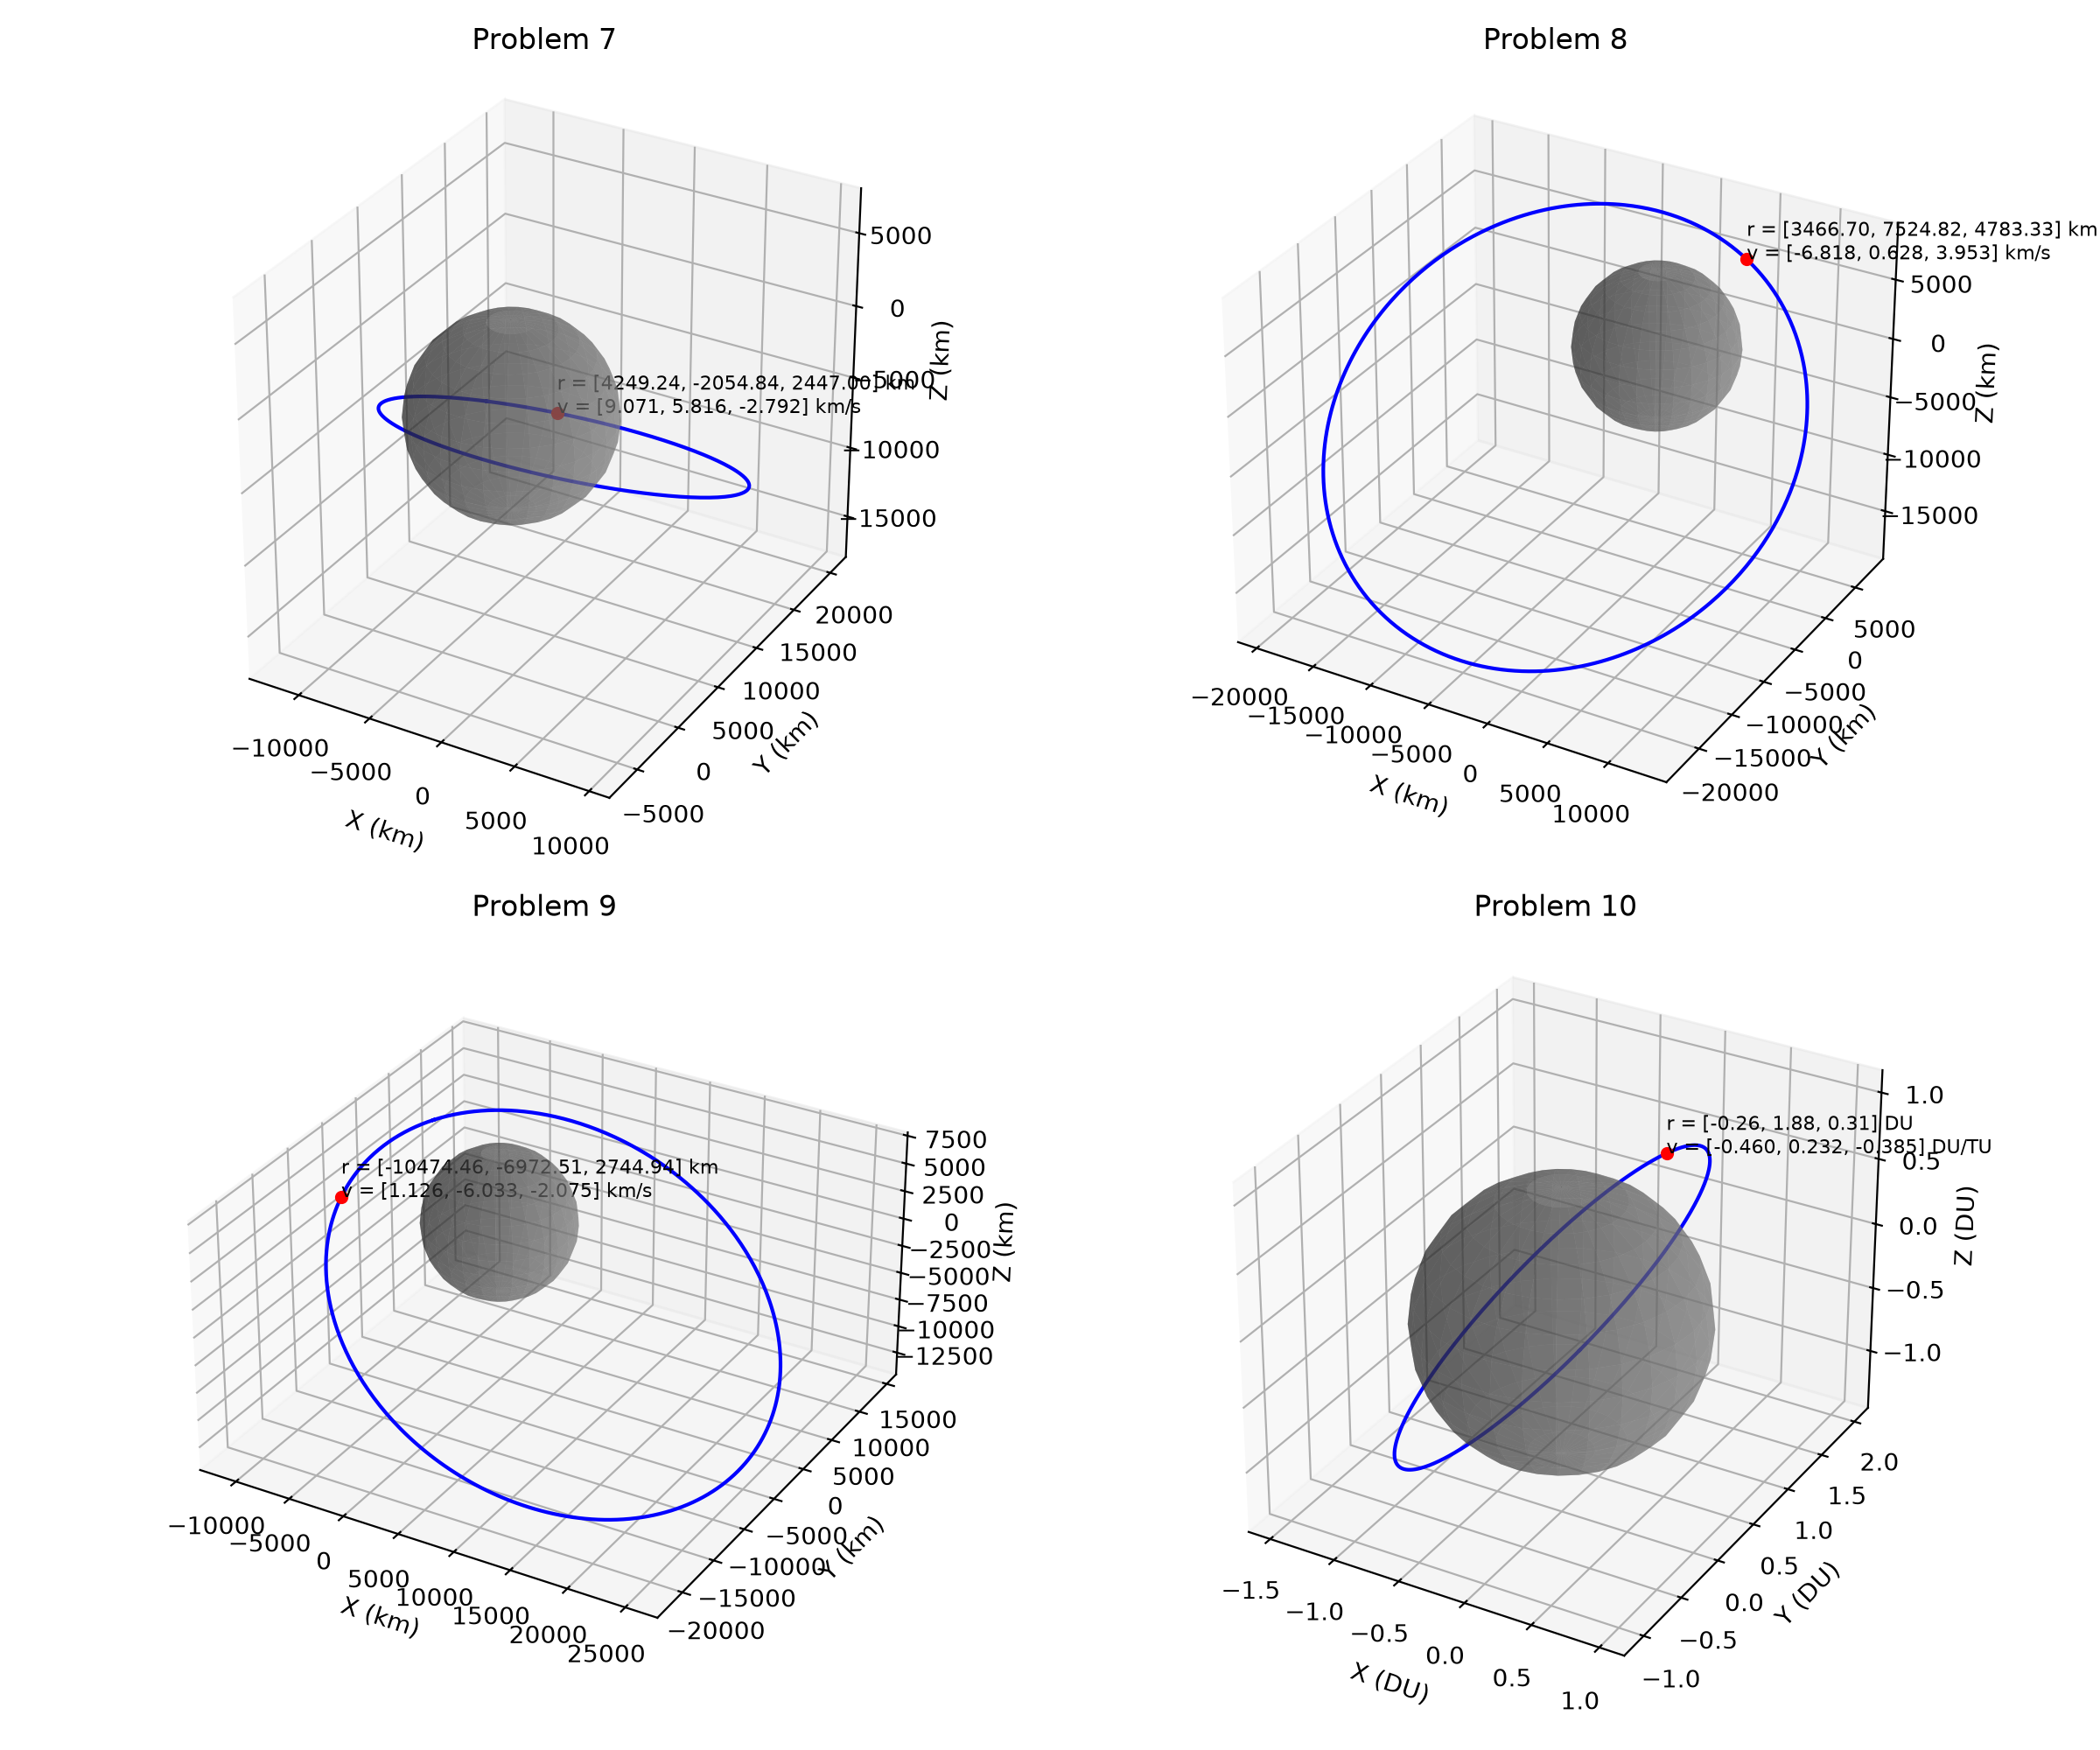
\includegraphics[width=\textwidth]{problems7to10_orbits.png}
\caption{Orbits for Problems 7 to 10 in planet-centered inertial coordinates. The planet (sphere of radius $R_E = 6378$ km, or 1 DU) is at the origin, and the spacecraft position (red) is labeled with its position and inertial velocity.}
\label{fig:p7-10}
\end{figure}

\FloatBarrier


\dividerpage{Appendices}{Python Source Code}{All code and sources found in: \repolink}
\appendix
\section{Python Source Code}
\label{app:code}

\subsection{Problem 1: \texttt{problem1.py}}
\label{app:p1-code}
\lstinputlisting[caption={Problem 1: position and velocity $\rightarrow$ orbital elements.}, label={lst:p1}]{../problem1.py}

\clearpage
\subsection{Problem 2: \texttt{problem2.py}}
\label{app:p2-code}
\lstinputlisting[caption={Problem 2: orbital elements $\rightarrow$ position and velocity (3--1--3 rotation).}, label={lst:p2}]{../problem2.py}

\clearpage
\subsection{Problem 5: \texttt{problem5.py}}
\label{app:p5-code}
\lstinputlisting[caption={Problem 5: asteroid orbital elements, $T$, $p$, $h$, $\mathcal{E}$ and impact check.}, label={lst:p5}]{../problem5.py}

\clearpage
\subsection{Problem 6: \texttt{problem6.py}}
\label{app:p6-code}
\lstinputlisting[caption={Problem 6: Problem 5 elements back to position and velocity.}, label={lst:p6}]{../problem6.py}

\clearpage
\subsection{Problems 7 to 10: \texttt{problems7to10.py}}
\label{app:p7-10-code}
\lstinputlisting[caption={Problems 7 to 10: position and velocity from orbital elements, and orbit plot.}, label={lst:p7-10}]{../problems7to10.py}


\end{document}
